%%%%%%%%%%%%%%%%%%%% book.tex %%%%%%%%%%%%%%%%%%%%%%%%%%%%%
%
% sample root file for the chapters of your "monograph"
%
% Use this file as a template for your own input.
%
%%%%%%%%%%%%%%%% Springer-Verlag %%%%%%%%%%%%%%%%%%%%%%%%%%


% RECOMMENDED %%%%%%%%%%%%%%%%%%%%%%%%%%%%%%%%%%%%%%%%%%%%%%%%%%%
\documentclass[pdftex,12pt, oneside]{article}

% choose options for [] as required from the list
% in the Reference Guide, Sect. 2.2
%\usepackage[paperwidth=8.5in, paperheight=13in]{geometry} % Folio
\usepackage[paperwidth=8.27in, paperheight=11.69in]{geometry} % A4

\usepackage{makeidx}         % allows index generation
\usepackage{graphicx}        % standard LaTeX graphics tool
                             % when including figure files
%\usepackage{multicol}        % used for the two-column index
\usepackage[bottom]{footmisc}% places footnotes at page bottom
\usepackage[english]{babel}
\usepackage{enumerate}
\usepackage{paralist}
\usepackage{float}
\usepackage{gensymb}  
\usepackage{listings}
\usepackage{hyperref}
%\usepackage{siunitx}
% etc.
% see the list of further useful packages
% in the Reference Guide, Sects. 2.3, 3.1-3.3
\renewcommand{\baselinestretch}{1.5}

\newcommand{\HRule}{\rule{\linewidth}{0.5mm}}

%\makeindex             % used for the subject index
                       % please use the style svind.ist with
                       % your makeindex program


%%%%%%%%%%%%%%%%%%%%%%%%%%%%%%%%%%%%%%%%%%%%%%%%%%%%%%%%%%%%%%%%%%%%%

\begin{document}

%\input{./01.title.tex}
\begin{center}
{\large STUDI KELAYAKAN RINCI PEMBANGUNAN LAYANAN SISTEM OTENTIKASI DI BADAN PENGELOLAAN PENDAPATAN, KEUANGAN DAN ASET DAERAH KABUPATEN BREBES}
\\[1cm]
22 Februari 2019\\
Priyanto Tamami, S.Kom.
\end{center}

\section{RUANG LINGKUP PEKERJAAN}

Ruang lingkup dari pekerjaan membangun sebuah sistem informasi otentikasi di Badan Pengelolaan Pendapatan, Keuangan dan Aset Daerah Kabupaten Brebes yaitu membangun sebuah sistem yang mampu melayani otentikasi termasuk otorisasi di dalamnya, untuk seluruh aplikasi yang berkaitan dengan Pajak Daerah di Kabupaten Brebes, adapun aplikasi atau sistem informasi yang akan dibangun berbasis \textit{web}, artinya untuk menggunakan aplikasi atau sistem informasi ini dibutuhkan \textit{browser} untuk menampilkan halaman sistem informasi.

Sistem informasi yang akan dibangun akan memiliki arsitektur dimana aplikasi yang dibangun akan dipisahkan menjadi 3 (tiga) bagian, yaitu bagian \textit{front-end} dan 2 (dua) bagian \textit{back-end}, bagian \textit{back-end} akan terdiri dari layanan sistem yang menyediakan otentikasi dan otorisasi itu sendiri, yang disebut \textit{Auth Server}, dan bagian lain akan melayani data yang digunakan untuk melakukan otentikasi dan otorisasi seperti informasi pengguna, informasi hak akses, dan informasi mengenai aplikasi klien yang dapat terhubung. Bagian \textit{front-end} dan bagian \textit{back-end} akan berkomunikasi melalui cara \textit{web service} dengan model REST. Data yang dikirim dari peladen \textit{web service} berupa JSON.

Pemilihan arsitektur ini karena nantinya aplikasi klien yang dapat terhubung dan menggunakan fasilitas otorisasi dan otentikasi bukan hanya aplikasi yang berbasis \textit{web}, namun termasuk juga aplikasi \textit{mobile} yang terpasang dalam ponsel pintar dan aplikasi yang berbasis \textit{desktop}.

Komunikasi data yang sifatnya universal dan mampu menghubungkan ketiga perangkat tersebut, yaitu peladen, klien berbasis aplikasi \textit{mobile} dan aplikasi berbasis \textit{desktop} adalah menggunakan arsitektur REST.

Bagian \textit{front-end} nantinya akan memiliki fungsi sebagai tampilan tatap muka untuk melakukan konfigurasi untuk tiap pengguna dan konfigurasi untuk tiap klien yang nantinya akan dihubungkan. Bagian \textit{front-end} nantinya akan terhubung ke 2 (dua) layanan di bagian \textit{back-end}, layanan yang pertama (yang disebut dengan \textit{OAuth Server}) tentu saja akan melakukan otorisasi dan otentikasi terhadap pengguna yang akan melakukan akses, layanan ini hanya menyediakan halaman masuk (\textit{login}) saja, yang kemudian, setiap aplikasi klien akan mendapatkan sebuah token yang digunakan untuk melakukan akses ke layanan yang kedua (yang diistilahkan sebagai \textit{resource server}). \textit{Resource server} inilah yang nantinya akan berkomunikasi dengan bagian \textit{front-end} (diistilahkan juga sebagai aplikasi klien) dalam penyediaan datanya. 

Untuk memastikan bahwa layanan pada \textit{Resource server} terlindungi, tiap permintaan (\textit{request}) yang dilakukan oleh aplikasi klien harus menyertakan token yang didapat dari proses otentikasi dengan \textit{OAuth Server}, nantinya token yang diterima oleh \textit{Resource server} dari aplikasi klien akan diverifikasi dengan melakukan verifikasi token.

Cara yang dilakukan \textit{Resource server} untuk memverifikasi token dari aplikasi klien adalah dengan melakukan dekripsi token menggunakan \textit{public key} yang disediakan oleh \textit{OAuth Server} yang dapat diakses secara bebas.

Token yang diimplementasikan sebagai tanda pengenal bahwa pengguna memiliki hak akses tertentu akan berbentuk JWT (\textit{JSON Web Token}) yang dijabarkan pada dokumen IETF (\textit{Internet Engineering Task Force}) dengan nomor RFC (\textit{Request for Comment}) 7519 yang telah diperbarui dengan dokumen IETF dengan nomor RFC 7797.

Sebagaimana dijelaskan dalam dokumen tersebut (IETF RFC No. 7519), bahwa JWT sebetulnya hanyalah sebuah teks (\textit{string}) yang mewakili beberapa pernyataan dari objek JSON yang terkode. Pernyataan dalam objek JSON sendiri adalah pasangan antara \textit{key} dan \textit{value}, dimana \textit{key} harus berupa teks (\textit{string}) dan \textit{value} dapat berupa nilai apapun yang dapat didefinisikan dalam JSON.

JSON sendiri sebetulnya adalah singkatan dari \textit{JavaScript Object Notation}, sebagaimana didefinisikan pada dokumen IETF (\textit{Internet Engineering Task Force}) dengan nomor RFC (\textit{Request for Comment}) 8259, bahwa JSON adalah sebuah format pertukaran data yang ringan, berbasis teks, dan independen terhadap bahasa pemrograman.

JSON sendiri dapat merepresentasikan 4 (empat) tipe data primitif seperti \textit{string}, \textit{number}, \textit{boolean}, dan \textit{null}, serta 2 (dua) tipe struktur, yaitu objek dan larik (\textit{array}).

\textit{String} sendiri adalah barisan dari 0 (nol) atau lebih karakter \textit{Unicode} yang tertuang pada laman \href{http://www.unicode.org/versions/latest/}{http://www.unicode.org/versions/latest/}. Harap dicatat bahwa petikan tersebut mengacu pada versi paling akhir dari \textit{Unicode} tanpa menyebutkan secara spesifik versinya. Karena hal ini, sehingga tidak menjamin bahwa perubahan yang terjadi pada spesifikasi \textit{Unicode} dimasa mendatang akan memiliki pengaruh terhadap sintak dari JSON.

\textit{Number} tentu saja adalah sebuah angka, baik bilangan bulat maupun pecahan, dan \textit{boolean} adalah tipe data primitif yang terdiri dari hanya 2 (dua) nilai, yaitu \textit{true} atau \textit{false}, sedangkan \textit{null} adalah tipe data yang menyatakan bahwa nilainya adalah kosong, atau data tanpa nilai.

Struktur Objek di JSON adalah himpunan yang tidak terurut yang terdiri dari 0 (nol) atau lebih pasangan \textit{name} dan \textit{value}, dimana \textit{name} adalah sebuah \textit{string} dan \textit{value} dapat berupa \textit{string}, \textit{number}, \textit{boolean}, \textit{null}, \textit{objek}, atau larik (\textit{array}).

Sedangkan struktur \textit{array} atau larik di JSON adalah barisan berurut yang terdiri dari 0 (nol) atau lebih nilai.

Bagian \textit{front-end} nantinya akan dibangun menggunakan \textit{framework} Angular, dan kedua bagian \textit{back-end}, baik \textit{OAuth Service} dan \textit{Resource Service} akan dibangun menggunakan Kotlin dan Springboot.

Hal-hal yang mendukung studi kelayakan dibangunnya sistem otentikasi dan otorisasi di Badan Pengelolaan Pendapatan, Keuangan, dan Aset Daerah ini yaitu dengan menggunakan metode analisis kelayakan TELOS (\textit{Technical}, \textit{Economic}, \textit{Legal}, \textit{Operational}, \textit{Schedule}).

Detail dari masing-masing faktor pada metode analisis kelayakan TELOS ini adalah seperti berikut :

\begin{enumerate}
	\item Faktor Kelayakan Teknis (\textit{Technical})
	
Kelayakan teknis menyoroti kebutuhan sistem yang telah disusun dari aspek teknologi yang digunakan, jika teknologi yang dikehendaki untuk pengembangan sistem merupakan teknologi yang mudah didapat, murah, dan tingkat pemakaiannya mudah, maka secara teknis usulan kebutuhan sistem bisa dinyatakan layak	
	
	\item Faktor Kelayakan Ekonomi (\textit{Economic})
	
Aspek yang paling dominan dari aspek kelayakan yang lain adalah kelayakan ekonomi. Tidak dapat disangkal lagi, motivasi pengembangan sistem informasi pada perusahaan atau organisasi adalah motif keuntungan. Dengan demikian aspek untung rugi jadi pertimbangan utama dalam pengembangan sistem. Kelayakan ekonomi berhubungan dengan \textit{return investmen} atau berapa lama biaya investasi dapat kembali, namun pada instansi pemerintah, yang secara umum bertugas melayani masyarakat, maka hubungannya bukan lagi untung rugi, tetapi lebih kepada imbas administrasi data yang tercatat dengan baik dan sedikit banyak mungkin berpengaruh pada peningkatan kepatuhan wajib pajak dalam memenuhi kewajiban pajaknya.	

% sampai sini
	
	\item Faktor Kelayakan Hukum (\textit{Legal})
	
Menguraikan secara hukum apakah sistem informasi yang akan dikembangkan tidak menyimpang dari hukum yang berlaku (tidak melanggar hukum jika diterapkan di objek penelitian). Misal: bagaimana kelayakan perangkat lunak yang digunakan, bagaimana kelayakan hukum informasi yang dihasilkan oleh program aplikasi yang dibuat. Apakah melanggar hukum atau tidak.	
	
	\item Faktor Kelayakan Operasional (\textit{Operational})

Penilaian terhadap kelayakan operasional digunakan untuk mengukur apakah sistem yang akan dikembangkan nantinya dapat dioperasikan dengan baik atau tidak untuk melayani masyarakat wajib pajak.	
	
	\item Faktor Kelayakan Jadwal \textit{Schedule})
	
Penilaian kelayakan jadwal ini digunakan untuk menentukan bahwa pengembangan sistem akan dapat dilakukan dalam batas waktu yang telah ditetapkan.	
	
\end{enumerate}

Adapun penilaian untuk masing-masing faktor kelayakan TELOS ini adalah sebagai berikut :

\begin{enumerate}
	\item Menilai kelayakan Teknik (\textit{Technical})
	
Kelayakan teknik menyoroti kebutuhan sistem yang telah disusun dari teknologi yang akan digunakan, untuk penerapan sistem informasi pembayaran untuk jenis pajak bumi dan bangunan sektor perdesaan dan perkotaan. Sistem informasi ini merupakan sistem berbasis \textit{web} yang digunakan oleh masyarakat wajib pajak melakukan verifikasi atau pengecekan pembayaran atas pajak terhutang. Sistem informasi dibangun berbasis \textit{web}, dengan tujuan agar seluruh wajib pajak dapat mengakses sistem informasi ini hanya dengan berbekal koneksi jaringan internet dan aplikasi \textit{browser} seperti Chrome, Firefox, Internet Explorer, Safari, atau jenis \textit{web browser} lainnya.

Sistem ini pun tidak memerlukan banyak \textit{input}, pengguna cukup memberikan informasi Nomor Objek Pajak pada kolom yang telah disediakan, sehingga target pengguna yang diharapkan yaitu pengguna yang tidak memiliki keahlian khusus komputer pun dapat mengoperasikan sistem ini.

\begin{enumerate}
	\item Kebutuhan Perangkat Keras, Perangkat Lunak, dan Perangkat Jaringan
	
\begin{enumerate}
	\item Perangkat Keras
	
Kebutuhan akan perangkat keras, sebetulnya tidak diperlukan pengadaan alat baru, melainkan dengan menggunakan perangkat yang sudah ada, sistem informasi ini akan dapat berjalan sebagaimana mestinya. Adapun perangkat keras yang digunakan adalah seperti berikut :

\begin{table}[H]
\centering
\begin{tabular}{| c | l | l |}
\hline
No & Perangkat keras & Keterangan \\
\hline
\multicolumn{3}{| c |}{\textit{Server} Aplikasi} \\
\hline
1 & Prosesor & Intel Xeon 2,4G 8 Core\\
\hline
2 & Memori & 8 GB \\
\hline
3 & Harddisk & \\
\hline
4 & Jaringan & 4 ethernet slot \\
\hline
\multicolumn{3}{| c |}{\textit{Server} Basis Data} \\
\hline
1 & Prosesor & Intel Xeon 2,4G 8 Core \\
\hline
2 & Memori & 32 GB \\
\hline
3 & Harddisk & \\
\hline
4 & Jaringan & 4 ethernet slot \\
\hline
\end{tabular}
\end{table}
	
	\item Perangkat Lunak
	
Kebutuhan akan perangkat lunak baru tentunya ada, tetapi tidak memerlukan biaya tambahan, karena beberapa perangkat lunak ada yang sudah terpasang, dan perangkat lunak yang akan di\textit{install} tidak memerlukan biaya tambahan.

\begin{table}[H]
	\centering
	\begin{tabular}{| c | l | l |}
		\hline
		No & Perangkat Lunak & Kegunaan \\
		\hline
		1 & Windows Server 2008 & Sistem Operasi \\
		\hline
		2 & Linux Ubuntu & Sistem Operasi \\
		\hline
		3 & IntelliJ IDEA & IDE \\
		\hline
		4 & Visual Studio Code & Editor \\
		\hline
		5 & Chrome, Firefox & Web Browser \\
		\hline
	\end{tabular}
\end{table}	
	
	\item Perangkat Jaringan
	
Kebutuhan akan perangkat jaringan pun tidak memerlukan pengadaan kembali, karena kondisi jaringan sudah terhubung dengan baik dengan peralatan seperti berikut :

\begin{table}[H]
	\centering
	\begin{tabular}{| c | l | l |}
		\hline
		No & Perangkat & Kegunaan \\
		\hline
		1 & Switch & Penghubung antar kabel jaringan \\ 
		\hline 
		2 & Kabel UTP & Media penghubung antar perangkat \\
		\hline
		3 & Konektor RJ-45 & Media penghubung antara kabel dengan \textit{socket} perangkat \\
		\hline
		4 & Modem & Sebagai perangkat penghubung jaringan lokal dan internet \\
		\hline
		5 & Router & Penghubung antar 2 atau lebih jaringan (berdasarkan alamat jaringan) \\
		\hline
	\end{tabular}
\end{table}	
	
\end{enumerate}	
	
	\item Arsitektur Jaringan Komputer
	
Arsitektur jaringan sistem informasi ini adalah seperti pada gambar \ref{fig:001-arsitektur-sistem}. Bila ada seorang pengguna yang melakukan akses dengan \textit{browser}, maka akan ditampilkan halaman 	utama dari sistem informasi ini. Akses ini oleh \textit{router} akan diarahkan ke \textit{server} aplikasi.

\begin{figure}[H]
	\centering
	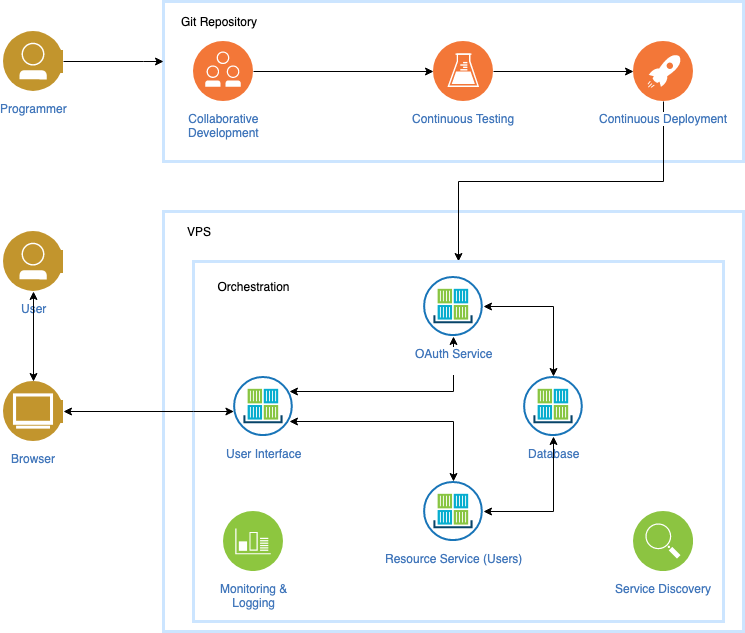
\includegraphics[width=1\textwidth]{./resources/arsitektur-sistem}
	\caption{Desain Arsitektur Sistem}
	\label{fig:001-arsitektur-sistem}
\end{figure}

Kemudian saat pengguna melakukan \textit{view} data terhadap nomor objek pajak tertentu, maka aplikasi akan melakukan \textit{request} data ke bagian \textit{back-end} yang selanjutnya bagian \textit{back-end} akan melakukan \textit{query} data ke sistem basis data. Setelah itu hasil yang didapatkan dari sistem basis data akan dikembalikan ke bagian \textit{front-end} untuk di olah dalam tampilan halaman \textit{web}.
	
\end{enumerate}

Adapun kondisi sistem informasi yang digunakan saat ini adalah seperti berikut :

\begin{enumerate}
	\item Sistem Aplikasi 
	
Aplikasi adalah sebuah \textit{tools} untuk membantu dan mempermudah suatu aktifitas administrasi maupun yang lainnya. Tanpa adanya aplikasi, tentu suatu aktifitas tidak bisa diselesaikan dengan cepat, segala sesuatunya dilakukan dengan pencatatan manual. Aplikasi atau sistem informasi yang digunakan di Badang Pengelolaan Pendapatan, Keuangan dan Aset Daerah Kabupaten Brebes saat ini adalah :

\begin{table}[H]
	\centering
	\begin{tabular}{| c | l | l |}
		\hline
		No & Aplikasi & Keterangan \\
		\hline
		1 & SISMIOP & Melakukan manajemen objek pajak PBB-P2 \\
		\hline
		2 & Microsoft Excel & Digunakan untuk mengolah data peralihan hak \\
		\hline
	\end{tabular}
\end{table}

Dengan adanya sistem informasi atau aplikasi tersebut, sudah membantu dari mulai manajemen pelayanan pajak bumi dan bangunan sektor perdesaan dan perkotaan, penetapan, penagihan, hinga ke prosedur pembayaran, namun demikian, sistem yang ada tidak memungkinkan informasi pembayarannya diakses oleh publik, maka dari itu dibutuhkan sistem atau aplikasi lain agar masyarakat wajib pajak mengetahui status pembayarannya, dengan tanpa melakukan prosedur instalasi apapun.
	
	\item Sistem Basis Data
	
Basis data merupakan suatu tempat penyimpanan data-data yang biasanya dari sebuah aplikasi, adapun basis data yang sudah ada pada Badan Pengelolaan Pendapatan, Keuangan dan Aset Daerah adalah seperti berikut :

\begin{table}[H]
	\centering
	\begin{tabular}{| c | l | l |}
		\hline
		No & Basis data & Keterangan \\
		\hline
		1 & Oracle DB & Digunakan untuk menyimpan data dari aplikasi SISMIOP \\
		\hline
		2 & SQL Server & Digunakan untuk menyimpan data dari aplikasi Simda Pendapatan \\
		\hline
	\end{tabular}
\end{table}	

Basis data yang digunakan masih belum terintegrasi dengan baik, karena penerimaan pembayaran pada SISMIOP belum dapat secara otomatis tercatat pada Simda Pendapatan. 

Sebetulnya sumber data yang digunakan pada pengelolaan Pajak Bumi dan Bangunan sektor Perdesaan dan Perkotaan ada pada 2 (dua) tempat, yang pertama berada di Badan Pengelolaan Pendapatan, Keuangan dan Aset Daerah Kabupaten Brebes, yang kedua berada di BPD Jateng.

Kondisi data yang berada di Badan Pengelolaan Pendapatan, Keuangan dan Aset Daerah berfungsi sebagai pendataan dan penetapan, namun realisasi pembayaran menggunakan data dari BPD Jawa Tengah. Selisih nilai antara 2 (dua) sumber data ini pasti terjadi, maka seharusnya dibutuhkan personil untuk melakukan pencocokan / rekonsiliasi data antara 2 (dua) sumber data tersebut agar data yang ditampilkan pada sistem informasi yang akan dibangun menjadi lebih lengkap.
	
	\item Infrastruktur
	
Infrastruktur merupakan sarana yang sangat dibutuhkan dalam sebuah aktifitas apapun termasuk aktifitas pengelolaan Pajak Daerah. Adapun infrastruktur yang ada pada Badan Pengelolaan Pendapatan, Keuangan dan Aset Daerah Bidang Pendataan dan Penetapan yaitu :

\begin{table}[H]
	\centering
	\begin{tabular}{| c | l | l |}
		\hline 
		No & Infrastruktur & Keterangan \\
		\hline
		1 & Komputer & Memiliki 13 komputer dan 4 \textit{server} \\
		\hline
		2 & Printer & Memiliki 4 \textit{printer multi-purpose}, 4 \textit{printer dot-matrix}, \\
		& & 3 \textit{printer line-matrix} \\
		\hline
		3 & Jaringan Internet & Memiliki 2 (dua) sumber internet, dengan 1 (satu) internet \\
		& & \textit{shared bandwidth} dan 1 (satu) internet \textit{dedicated} \\
		\hline
	\end{tabular}
\end{table}

Dari kondisi infrastruktur di atas, sebetulnya Badan Pengelolaan Pendapatan, Keuangan dan Aset Daerah cukup untuk membuka atau melayani sebuah sistem informasi status pembayaran Pajak Bumi dan Bangunan Sektor Perdesaan dan Perkotaan yang akan dibangun.

Melihat kondisi teknis demikian, dimana sistem belum pernah dibuat, teknologi yang digunakan terbilang cukup baru, sehingga nilai kelayakan teknik yang dapat diberikan adalah 9.0.
	
\end{enumerate}
	
	\item Menilai kelayakan Ekonomi (\textit{Economic})
	
Pembangunan sistem baru tentunya membutuhkan investasi ataupun dana yang tidak sedikit, untuk mendapatkan manfaat dimasa yang akan datang, sumber daya dan sumber dana diperlukan dalam pembangunan sistem baru sebagai bentuk investasi.

Untuk menganalisis kelayakan ekonomi digunakan kalkulasi analisis biaya dan manfaat (\textit{cost benefit analysis}). Adapun tujuan dari analisis biaya dan manfaat adalah untuk memberikan gambaran kepada internal Badan Pengelolaan Pendapatan, Keuangan dan Aset Daerah, apakah manfaat yang diperoleh dari sistem baru "lebih besar" dibandingkan dengan biaya yang dikeluarkan. 

Pada analisis biaya dan manfaat ada beberapa metode kuantitatif yang digunakan untuk menemukan standar kelayakan proyek.

\textbf{Analisis Biaya dan Manfaat}

Untuk melakukan analisa biaya dan manfaat diperlukan dua komponen, yaitu komponen biaya dan komponen manfaat.

\begin{enumerate}
	\item Komponen Biaya
	
Biaya yang berhubungan dengan pembuatan sistem ini dapat diklasifikasikan ke dalam 3 (tiga) kategori utama, yaitu :

\begin{enumerate}
	\item Biaya pengadaan, yaitu biaya pembelian perangkat keras, yang digunakan pada awal pembuatan sistem, sebelum sistem dioperasikan.
	\item Biaya Pengembangan, yaitu biaya pembuatan perangkat lunak sistem yang meliputi biaya konsultasi, biaya tahap analisa sistem, biaya tahap desain sistem dan biaya tahap penerapan sistem.
	\item Biaya operasi dan biaya perawatan, yaitu biaya yang dikeluarkan untuk menjalankan sistem, yaitu biaya \textit{overhead}, biaya perawatan terhadap perangkat keras dan perangkat lunak.
\end{enumerate}	
	
	\item Komponen Manfaat.
	
Manfaat yang didapat dari sistem informasi diklasifikasi sebagai berikut :

\begin{enumerate}
	\item Keuntungan berwujud adalah keuntungan yang berupa penghematan atau peningkatan di dalam pengelolaan pajak daerah yang dapat diukur dalam bentuk satuan nilai uang. Keuntungan berwujud antara lain :
	
	\begin{enumerate}
		\item Pengurangan biaya cetak
		\item Pengurangan biaya operasi
		\item Pengurangan biaya perlengkapan
	\end{enumerate}
	
	\item Keuntungan tak berwujud, adalah keuntungan yang sulit atau tidak mungkin diukur dalam bentuk satuan uang. Keuntungan tersebut antara lain :
	
	\begin{enumerate}
		\item Peningkatan kepatuhan wajib pajak
		\item Peningkatan efektifitas pegawai
		\item Peningkatan kepuasan masyarakat
	\end{enumerate}
\end{enumerate}	

Adapun metode untuk melakukan analisis biaya dan manfaat adalah :

\begin{enumerate}
	\item Metode Periode Pengembalian

Metode ini adalah uji kuantitatif yang digunakan untuk menghitung jangka waktu yang diperlukan untuk membayar kembali biaya investasi dalam pembuatan aplikasi yang telah dikeluarkan. Penilaian kelayakan untuk pengembalian 

\[periode = \frac{investasi}{proceed} x tahun \]

\begin{enumerate}
	\item Layak jika waktu pengembalian lebih kecil dari umur investasi
	\item Tidak layak jika waktu pengembalian lebih besar dari umur investasi.
\end{enumerate}

Perhitungan Periode Pengembalian adalah seperti berikut :

Nilai Investasi = Rp0,-
Proses Th 1 = Rp30.000.000.000,-

Nilai investasi memang bernilai 0 (nol) rupiah karena seluruh sarana dan prasarana telah tersedia, hanya tinggal membangun sebuah sistem informasi untuk digunakan dan dijalankan. Sedangkan nilai Rp30.000.000.000,- (Tiga puluh milyar) didapat dari nilai target penerimaan jenis pajak bumi dan bangunan sektor perdesaan dan perkotaan.

\[ PP = \frac{0}{30.000.000.000} \]

\[ PP = 0 tahun \]

Artinya, karena nilai investasi yang dikeluarkan nihil sama sekali, atau dengan kata lain tidak memerlukan nilai investasi, namun sistem informasi secara tidak langsung memberikan andil terhadap realisasi sebesar 30 Milyar Rupiah kepada Kas Daerah. Artinya sistem ini sangat layak untuk dikembangkan karena pengembalian tidak membutuhkan waktu untuk mencapai titik impas.
	
	\item Metode Pengembalian Investasi
	
Metode pengembalian investasi digunakan untuk mengukur presentase manfaat yang dihasilkan proyek dibandingkan dengan biaya yang dikeluarkan.

\textit{Return On Investmen} (ROI) dari suatu proyek dapat dihitung dengan rumus penilaian kelayakan untuk ROI :

\begin{enumerate}
	\item Layak jika ROI $>$ 0
	\item Tidak layak jika ROI $<$ 0
\end{enumerate}	

\[ ROI = \frac{Total Manfaat - Total Biaya}{Total Biaya} x 100\% \]
	
Karena nilai biaya tidak akan pernah muncul, maka bisa disebut bahwa Total Biaya = 0 (nol), Total Manfaat adalah penerimaan realisasi Pajak Bumi dan Bangunan sektor Perdesaan dan Perkotaan dalam satu tahun pajak, yaitu senilai 30 Milyar rupiah. Maka hasil yang didapatkan adalah seperti berikut :

\[ ROI = \frac{30 M - 0}{0} x 100\% \]

\[ ROI = \infty \]

Ternyata karena kondisi pembaginya adalah 0 (nol), maka hasil yang didapatkan menghasilkan Tak Terhingga. Ini dikarenakan bilangan pembagi adalah 0 (nol) sehingga menghasilkan nilai demikian, artinya proyek apapun itu bila tidak memerlukan biaya sama sekali, namun bisa mendapatkan manfaat maksimal tentunya ini proyek dengan ROI tak terhingga.

Jadi, karena nilai $ \infty $ itu lebih dari 0 (nol) maka proyek ini layak untuk dikerjakan.
	
	\item Metode Nilai Sekarang Bersih
	
Metode nilai sekarang bersih merupakan metode yang memperhatikan nilai waktu dari uang. Suku bunga diskonto mempengaruhi arus dari uangnya (\textit{proceed}). Metode Nilai Sekarang Bersih atau lebih dikenal dengan \textit{Net Present Value} (NPV) dapat dihitung dari selisih nilai proyek pada awal tahun dikurangi dengan \textit{proceed} tiap tahun yang dinilai uangkan ketahun awal dengan tingkat bunga diskonto.

Kriteria NPV ini adalah seperti berikut :

\begin{itemize}
	\item NPV $>$ 0 : \textit{Feasible}
	\item NPV = 0 : \textit{Indifferent}
	\item NPV $<$ 0 : \textit{Unfesible}
\end{itemize}

Rumus untuk menghitung NPV ini adalah seperti berikut :

\[ NPV = - NilaiProyek + \frac{proceed1}{(1 + i)^1} + \frac{proceed2}{(1 + i)^2} + \frac{proceedn}{(1 + i)^n} \]

dimana :

\begin{itemize}
	\item i adalah tingkat bunga diskonto diperhitungkan
	\item n adalah umur proyek investasi
	\item proceed adalah selisih biaya dan manfaat
\end{itemize}

Sehingga perhitungannya dapat kita cari seperti berikut :

\[ NPV = - 0 + \frac{30 M}{(1 + 6.5\%)^1} \]

\[ NPV = - 0 + \frac{30 M}{1.065} \]

\[ NPV =  28.169.014.084.51 \]
Pada perhitungan di atas, nilai waktu dari bunga uang yang ditanamkan adalah 6,5\% berdasarkan suku bunga dari www.bi.go.id pada tanggal 21 Juli 2016. Karena nilai NPV $>$ 0 berarti investasi dapat diterima dan layak untuk dikembangkan.
	
\end{enumerate}

Dengan melihat ketiga metode untuk kelayakan ekonomi maka dapat dikatakan bahwa sistem informasi yang akan dibangun layak dan dapat dikerjakan sebagaimana mestinya. Nilai yang diberikan untuk kelayakan ekonomi ini adalah 9,0.
	
\end{enumerate}
	
	\item Menilai kelayakan Hukum (\textit{Legal})
	
Kelayakan hukum adalah kelayakan yang berkaitan dengan legalitas atau kekuatan hukum. Berarti bahwa sistem informasi yang akan dibangun tidak boleh melanggar hukum yang berlaku, baik hukum yang ditetapkan oleh pemerintah maupun hukum yang ditetapkan berdasarkan peraturan-peraturan organisasi. 

Proyek pembangunan sistem informasi yang akan dikembangkan secara hukum dinilai layak karena perangkat lunak (\textit{software}) yang digunakan resmi sesuai dengan perijinan yang ada, karena sebagian besar menggunakan perangkat lunak yang bersifat \textit{free} atau gratis.

Adapun rincian perangkat lunak secara hukum adalah sebagai berikut :

\begin{table}[H]
\centering
\begin{tabular}{| c | l | l |}
	\hline
	No & \textit{Software} & Lisensi \\
	\hline
	1 & Windows Server 2008 R2 & Lisensi tersedia \\
	\hline
	2 & Linux Ubuntu & Gratis \\
	\hline
	3 & Intellij IDEA Community Edition & Gratis, Apache 2.0 \\
	\hline
	4 & Visual Studio Code & Gratis, MIT \\
	\hline
	
\end{tabular}
\end{table}

Karena sistem informasi yang akan dibangun tidak meliputi data sensitif, seperti data detail wajib pajak, dan pada saat melakukan akses diperlukan Nomor Objek Pajak yang hanya wajib pajak saja yang memiliki, sehingga nilai untuk kelayakan hukum ini adalah 9,0.
	
	\item Menilai kelayakan Operasional (\textit{Operational})
		
Kelayakan operasional dinilai dengan menggunakan kerangka kerja PIECES yang merupakan singkatan dari \textit{Performance}, \textit{Information}, \textit{Economy}, \textit{Control}, \textit{Efficiency}, dan \textit{Services}. Kerangka kerja PIECES ini dikembangkan oleh James Wetherbe yang bertujuan mengukur apakah sistem yang akan dikembangkan dapat dioperasikan dengan baik atau tidak di dalam organisasi.

Penjelasan untuk masing-masing poin dalam kerangka kerja PIECES ini adalah seperti berikut ini :

\begin{itemize}
	\item \textit{Performance} atau kinerja adalah untuk mengetahui apakah sistem menyediakan \textit{throughput} dan \textit{response time} yang cukup. Perbandingannya adalah seperti berikut ini :
	
	\begin{table}[H]
		\centering
		\begin{tabular}{| p{7cm} | p{7cm} |}
			\hline
			Sistem Lama & Sistem Baru \\
			\hline
			Waktu yang dibutuhkan untuk melakukan pengambilan data pembayaran untuk tiap Nomor Objek Pajak membutuhkan waktu cukup lama karena banyaknya menu & Waktu yang dibutuhkan untuk mencari informasi objek pajak berdasarkan Nomor Objek Pajak relatif singkat. \\
			\hline
		\end{tabular}
	\end{table}
	
\item \textit{Information} atau informasi adalah untuk mengetahui apakah sistem menyediakan informasi yang berkualitas bagi pengguna. 

\begin{table}
	\centering
	\begin{tabular}{| p{7cm} | p{7cm} |}
		\hline
		Sistem Lama & Sistem Baru \\
		\hline
		Informasi yang disajikan hanya dapat diakses oleh pegawai internal dan melalui aplikasi \textit{desktop} & Informasi dapat diakses oleh siapa saja pemegang Nomor Objek Pajak \\
		\hline
	\end{tabular}
\end{table}

\item \textit{Economy} atau ekonomi adalah untuk mengetahui apakah sistem menawarkan tingkat dan kapasitas pelayanan yang memadai untuk mengurangi biaya dan meningkatkan keuntungan. Berikut adalah perbandingan dari sistem lama dan baru :

\begin{table}	
	\centering
	\begin{tabular}{| p{7cm} | p{7cm} |}
		\hline 
		Sistem Lama & Sistem Baru \\
		\hline
		Biaya yang dikeluarkan tinggi, karena terkadang wajib pajak meminta versi cetak-nya & Biaya yang dikeluarkan relatif rendah, karena wajib pajak dapat melakukan akses mandiri terhadap datanya. \\
		\hline		
	\end{tabular}
\end{table}

\item \textit{Control} atau pengendalian adalah untuk mengetahui apakah sistem informasi yang dibangun menawarkan kontrol atau pengendalian untuk mengatasi kecurangan-kecurangan dan untuk menjamin keakuratan dan keamanan data. Berikut adalah perbandingan sistem yang lama dan sistem yang baru :

\begin{table}[H]
	\centering
	\begin{tabular}{| p{7cm} | p{7cm} |}
	 	\hline
		Sistem Lama & Sistem Baru \\
		\hline
		Hanya dapat diakses oleh pengguna yang terdaftar pada sistem informasi SISMIOP & Data dapat diakses oleh siapapun yang mengetahui Nomor Objek Pajak yang akan dicari \\
		\hline
	\end{tabular}
\end{table}

Namun akses datanya hanya dapat dilihat saja, tidak dapat merubah data yang ditampilkan.

\item \textit{Efficiency} atau efisiensi adalah untuk mengetahui apakah sistem menggunakan secara maksimum sumber yang tersedia termasuk orang, waktu aliran \textit{form}, meminimalkan penundaan proses. Berikut adalah perbandingan sistem informasi yang lama dan sistem informasi yang baru :

\begin{table}[H]
	\centering
	\begin{tabular}{| p{7cm} | p{7cm} |}
		\hline
		Sistem Lama & Sistem Baru \\
		\hline
		Wajib pajak harus datang ke kantor hanya untuk mengetahui status pembayaran atau perubahan nama pada Surat Pemberitahuan Pajak Terhutangnya & Wajib pajak dapat melakukan pemeriksaan secara mandiri terhadap data miliknya berdasarkan Nomor Objek Pajak. \\
		\hline
	\end{tabular}
\end{table}

\item \textit{Services} atau pelayanan adalah untuk mengetahui apakah sistem menyediakan layanan yang diinginkan dan handal pada siapa saja yang menginginkannya, dan apakah sistem fleksibel dan dapat dikembangkan. Berikut adalah perbandingannya antara sistem lama dan sistem baru :

\begin{table}[H]
	\centering
	\begin{tabular}{| p{7cm} | p{7cm} |}
		\hline
		Sistem Lama & Sistem Baru \\
		\hline
		Pelayanan sangat membebani wajib pajak yang harus datang ke kantor dan mengantri bila ada antrian hanya untuk mengetahui data pembayarannya & Wajib pajak cukup melakukan akses dari mana pun berdasarkan Nomor Objek Pajak untuk mengetahui data pembayarannya \\
		\hline
	\end{tabular}
\end{table}
	
\end{itemize}

Karena sistem berbasis \textit{web} dan banyak pengguna, serta tidak memerlukan keahlian khusus untuk melakukan operasinya. Maka nilainya kita berikan 7,0.
	
	\item Menilai kelayakan Jadwal (\textit{Schedule})
	
Kelayakan jadwal digunakan untuk menentukan bahwa pengembangan sistem dapat dilakukan dalam batas waktu yang telah ditetapkan. Pengembangan sistem direncanakan selesai dalam waktu maksimal $\pm$ 9 minggu. Adapun perkiraan tahap-tahap pengembangan sistem dijadwalkan sebagai berikut :

Dalam proyek pengembangan sistem informasi Pembayaran Pajak Bumi dan Bangunan Sektor Perdesaan dan Perkotaan dilakukan dalam 9 (sembilan) tahap, yaitu :

\begin{enumerate}
	\item Tahap analisa kebutuhan sistem 
	\item Tahap studi kelayakan
	\item Tahap desain \textit{user interface}
	\item Tahap desain data
	\item Tahap desain \textit{proses}
	\item Tahap Pengodean
	\item Tahap persiapan tempat \textit{instalasi}
	\item Tahap \textit{instalasi} perangkat keras dan perangkat lunak
	\item Tahap uji sistem
	\item Tahap dokumentasi
\end{enumerate}

Grafik \textit{Gantt} untuk tahapan-tahapan tersebut adalah seperti pada gambar \ref{fig:002-gantt-chart} berikut ini :

\begin{figure}[H]
	\centering
	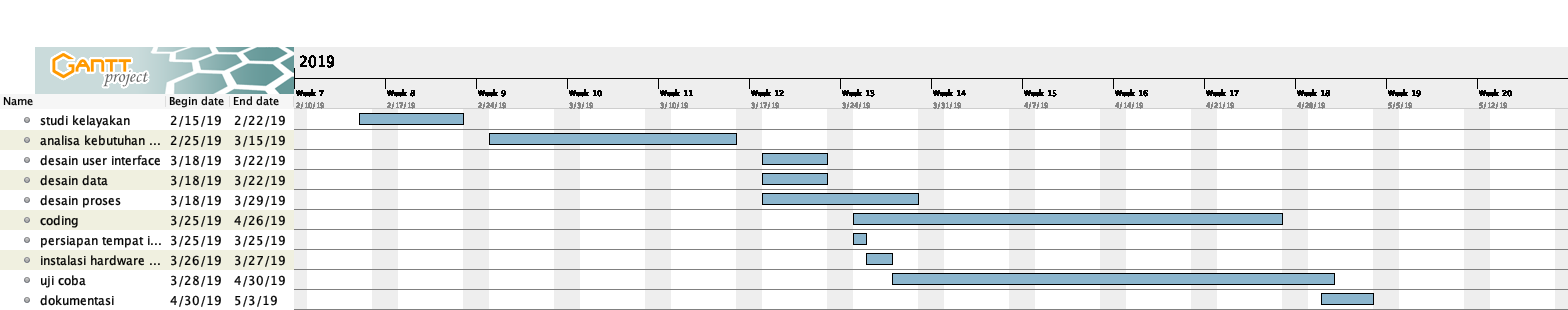
\includegraphics[width=1\textwidth]{./resources/gantt-chart}
	\caption{Grafik \textit{Gantt}}
	\label{fig:002-gantt-chart}
\end{figure}

Karena pengembangan diukur dalam jam, hari, minggu, dan bulan maka kesalahan perkiraan (\textit{error estimation}) yang dibutuhkan untuk perancangan dan implementasi menjadi kecil. Maka nilainya 8.0
	
\end{enumerate}

Dari keseluruhan faktor kelayakan TELOS tersebut, jumlah dari semua faktornya adalah 

\[ Total = 9 + 9 + 9 + 7 + 8 \]

\[ Total = 44 \]

Total score dari kelayakan ini adalah :

\[ score = 44 / 5 = 8,8 \]

Artinya perancangan pengembangan sistem informasi yang dievaluasi adalah LAYAK dengan resiko pengembangan sistem informasi yang cukup rendah.

\section{SARANA DAN PRASARANA YANG MELIPUTI PERANGKAT KERAS DAN PERANGKAT LUNAK YANG DIPERLUKAN}

Kebutuhan akan sarana dan prasarana untuk jenis perangkat keras yaitu :

\begin{enumerate}
	\item Peladen (\textit{server}) Basis Data
	
Peladen atau \textit{server} ini berfungsi untuk menyimpan basis data hasil proses penetapan yang menghasilkan nilai pajak terhutang untuk pajak bumi dan bangunan sektor perdesaan dan perkotaan, untuk nantinya dapat diakses oleh peladen (\textit{server}) aplikasi \textit{web} yang menyediakan sebuah API (\textit{Application Programming Interface}) untuk diakses oleh aplikasi \textit{web} dan aplikasi \textit{mobile} yang juga akan dibangun.

Kebutuhan perangkat keras peladen ini tidak perlu membeli karena nantinya akan menggunakan peladen yang sudah ada sebagai peladen basis data untuk aplikasi SISMIOP (Sistem Manajemen Informasi Objek Pajak) yang sudah beroperasi.
	
	\item Peladen (\textit{server}) \textit{web} aplikasi
	
Peladen ini akan digunakan sebagai tempatnya aplikasi \textit{web} yang menyediakan API (\textit{Application Programming Interface})	untuk aplikasi \textit{web} Angular dan aplikasi \textit{mobile}.

Peladen ini juga akan menjadi tempat aplikasi \textit{web} bagian ujung depan (\textit{front-end}) berada. Aplikasi ujung depan (\textit{front-end}) dengan aplikasi ujung belakang (\textit{back-end}) yang bisa kita sebut peladen API (\textit{Application Programming Interface}) adalah 2 (dua) aplikasi yang berbeda fungsi, berbeda bahasa pemrograman, yang dibangun secara mandiri tetapi saling berkomunikasi dalam sebuah sistem.

Peladen ini pun tidak perlu membeli karena nantinya akan menggunakan peladen yang sudah disediakan sebagai peladen aplikasi \textit{web}.
	
	\item Kartu Jaringan
	
Kartu jaringan digunakan atau terpasang pada peladen agar peladen dapat terhubung dengan jaringan, baik jaringan LAN (\textit{Local Area Network}) maupun jaringan \textit{internet}. 

Kartu jaringan ini tidak perlu membeli karena sudah terpasang lebih dari 1 (satu) pada tiap peladen yang dapat dikonfigurasi secara mandiri seluruhnya.
	
	\item Kabel \textit{Unshielded Twisted Pair} (UTP)
	
Kabel ini terdiri dari 4 (empat) pasang warna yang digunakan sebagai penghubung atau media komunikasi antar kartu jaringan yang terdapat pada tiap peladen agar aplikasi atau data pada peladen dapat diakses melalui jaringan.

Kabel ini juga tidak perlu membeli karena telah terpasang dan saling terhubung dari tiap peladen ke area jaringan.	
	
	\item Konektor RJ45
	
Konektor ini digunakan atau dipasangkan pada kabel UTP agar kabel UTP dapat dipasangkan pada kartu jaringan di tiap peladen dan tiap perangkat jaringan seperti \textit{switch}, \textit{router}, ataupun \textit{modem}. 

Masing-masing helai kabel UTP akan terpasang pada tiap pin yang ada pada konektor RJ45, yang kemudian apabila konektor RJ45 dipasangkan pada kartu jaringan, atau slot RJ45 yang terdapat pada \textit{switch}, \textit{router} ataupun \textit{modem}, akan terhubung dengan pin pada RJ45 sehingga aliran data dapat disampaikan dari 1 (satu) peladen ke perangkat jaringan yang lain.	
	
	\item \textit{Switch}
	
Masing-masing komponen yang terkoneksi / terhubung ke jaringan dapat diistilahkan sebagai \textit{host}, tentunya untuk membuat agar 1 (satu) \textit{host} terhubungan dengan 1 (satu) \textit{host} yang lain maka diperlukan sebuah kartu di masing-masing	\textit{host} dan sebuah kabel jaringan yang sudah terpasang konektor RJ45. Akan menjadi masalah apabila ada lebih dari 2 (dua) \textit{host} yang perlu terhubung. Rumusnya akan menjadi demikian :

	\begin{enumerate}
		\item Untuk mengetahui jumlah kebutuhan kartu jaringan yaitu menggunakan rumus :

\[ JumlahKartuJaringan = n(n - 1) \]		

dimana \texttt{n} adalah jumlah \textit{host}

		\item Sedangkan untuk mengetahui jumlah kabel jaringan yaitu menggunakan rumus :
		
\[ JumlahKabelJaringan = \frac{n(n-1)}{2} \]

dimana \texttt{n} adalah jumlah \textit{host}
		
	\end{enumerate}
	
Ini akan lebih efektif dan efisien apabila digunakannya \textit{switch} sebagai penghubung atau pengatur lalu lintas data antar \textit{host}. Sebagai contoh bila ada 2 (dua) \textit{host} yang akan dihubungkan dengan jaringan menggunakan \textit{switch} ini, maka diperlukan 1 (satu) buah \textit{switch}, 2 (dua) buah kabel jaringan (UTP), dan 2 (dua) buah kartu jaringan.

Bagaimana bila ada 3 (tiga) atau lebih \textit{host} yang akan dihubungkan dalam sebuah jaringan yang sama, maka cukup menggunakan 1 (satu) buah \textit{switch}, \texttt{n} buah kabel jaringan (UTP) dan \texttt{n} buah kartu jaringan sebanyak jumlah \textit{host} yang akan dihubungkan. Tentunya model \textit{switch} perlu disesuaikan jumlah \textit{port} dengan jumlah \textit{host} yang akan dihubungkan.

\textit{Switch} ini selain menjadikan jaringan komputer lebih efektif dan efisien, juga mengatur lalu lintas data secara lebih baik (dibandingkan \textit{hub}). Salah satu kelebihan yang dimiliki \textit{switch} dibanding \textit{hub} adalah data akan disampaikan tepat kepada alamat yang dituju, sehingga pertukaran data nyaris aman dalam jalur komunikasinya, sedangkan \textit{hub} lebih rentan karena setiap data yang data yang terkirim dan dilewatkan melalui \textit{hub}, maka alat ini akan menyebarkan berita ke setiap \textit{host} yang terhubung dengan \textit{hub} yang kemudian diserahkan kepada kartu jaringan apakah data yang diterima sesuai dengan alamat yang dimiliki atau tidak. Dalam kondisi ini, keamanan data akan terlalu berresiko saat terjadi komunikasi.

\textit{Switch} ini pun tidak perlu membeli karena sudah terpasang pada sistem yang lama sebagai penghubung antar 1 (satu) \textit{host} dengan \textit{host} yang lain.
	
	\item \textit{Router}
	
Alat ini dalam istilah lain juga disebut sebagai gerbang (\textit{gateway}), yaitu sebuah jembatan yang menghubungkan 2 (dua) atau lebih jaringan yang berbeda alamat, cara kerja alat ini yaitu dengan memiliki peta \textit{routing} yang diprogram, peta inilah yang dibaca oleh \textit{router} kemana paket data yang diterima harus dikirimkan, apabila tujuan paket data hanya dikirimkan untuk \textit{host} yang berada di jaringan lokal, maka \textit{router} tidak akan mengirimkan paket datanya keluar, melainkan akan dikirim ke alamat yang berada di dalam jaringan LAN (\textit{Local Area Network}), tetapi bila tujuan paket data berada di luar jaringan, maka paket tersebut akan dikirimkan ke jaringan lain dalam lingkupnya, atau diteruskan ke \textit{router} lain yang menghubungkan jaringan di luar lingkupnya.

Tentunya cara kerja tersebut di atas dengan konfigurasi peta jaringan yang sebelumnya sudah diatur dalam \textit{router}. Dan biasanya, pada setiap \textit{router} terdapat \textit{firewall} yang akan memberikan proteksi atau aturan-aturan komunikasi, dimana tidak semua data dapat diteruskan ke jaringan lain di luarnya, tetapi harus memenuhi persyaratan yang ditetapkan dalam tabel \textit{firewall}.

Jaringan internal atau LAN pada bidang Pendataan dan Penetapan memiliki sebuah alamat jaringan lokal baik untuk jaringan nirkabel atau jaringan dengan kabel (UTP) di alamat 192.168.2.0/24, sedangkan untuk terhubung dengan internet digunakan sebuah \textit{router} yang akan menjembatani atau menjadi gerbang antara jaringan internet dengan jaringan pada LAN. \textit{Router} ini pula yang nantinya akan meneruskan data dan melakukan filter data baik yang masuk dari jaringan internet yang aksesnya atau \textit{request}-nya akan diteruskan ke peladen aplikasi \textit{web}.

Dengan kondisi demikian, maka biaya pengadaan untuk \textit{router} sendiri tidak diperlukan, karena sudah terpasang dan sudah digunakan untuk kegiatan komunikasi data pada jaringan yang sudah ada sebelumnya.
	
	\item \textit{Modem}
	
Fungsi dari \textit{modem} yaitu untuk menghubungkan 2 (dua) atau lebih media jaringan yang berbeda sehingga data dapat dikomunikasikan pada jaringan yang berbeda media tersebut. Sebagai contoh, karena bidang Pendataan dan Penetapan menggunakan akses serat-optik (\textit{fiber optik}) dari jaringan penyedia layanan internet, dan jaringan internal menggunakan kabel UTP, maka dibutuhkan \textit{modem} untuk menerjemahkan data yang melintas melalui 2 (dua) media jaringan tersebut.

Karena \textit{modem} ini sudah digunakan pada sistem jaringan sebelumnya, maka tidak perlu dibeli.
	
\end{enumerate}

Sehingga kebutuhan perangkat keras secara keseluruhan sebetulnya tidak perlu mengeluarkan biaya tambahan lain karena perangkat-perangkat tersebut sudah tersedia dan cukup untuk mengakomodir berjalannya sistem informasi yang nantinya akan dibangun.

Kemudian, untuk sarana dan prasarana jenis perangkat lunak yang dibutuhkan yaitu :

\begin{enumerate}
	\item Perangkat Lunak Sistem Operasi
	
Perangkat lunak sistem operasi digunakan sebagai dasar dari seluruh sistem yang akan berjalan diatasnya. Pemilihan sistem operasi ini pun harus dapat memenuhi kriteria stabil dalam melakukan tugasnya sebagai peladen untuk rentang waktu 24 jam selama 7 hari berturut-turut.

Tentunya sistem operasi ini sudah terpasang baik pada peladen-peladen yang nantinya akan menjadi peladen sistem basis data dan peladen aplikasi \textit{web}. Pada peladen sistem basis data terpasang sistem operasi Windows Server 2008 R2 dengan lisensi legal yang sah tersedia karena hasil pengadaan di tahun sebelumnya. Sedangkan pada peladen aplikasi \textit{web} telah terpasang sistem operasi Ubuntu Server 14.04 yang tentu saja, untuk sistem operasi ini berlisensi gratis sehingga kebutuhan akan kedua peladen ini tidak perlu mengeluarkan biaya tambahan baik untuk lisensinya maupun pemasangannya.
	
	\item Perangkat Lunak Sistem Basis Data
	
Perangkat lunak basis data digunakan sebagai sistem yang nantinya akan mengatur dan menyimpan data-data hasil perekaman yang dilakukan oleh petugas pelayanan dan petugas entri data, yang kemudian hasil perekaman ini dapat diolah untuk menyajikan berbagai macam laporan yang nantinya diproduksi dan dibutuhkan oleh aplikasi \textit{web}, termasuk di antaranya adalah aplikasi yang akan dibangun ini.

Pemilihan perangkat lunak basis data ini pun dikarenakan pada saat pengelolaan pajak bumi dan bangunan sektor perdesaan dan perkotaan di kelola oleh Pemerintah Pusat, aplikasi di bangun dan datanya di simpan dalam sistem basis data Oracle, sehingga pada saat persiapan pengalihan pajak bumi dan bangunan sektor perdesaan dan perkotaan menjadi pajak daerah, maka dibeli juga lisensi sistem basis data Oracle agar migrasi data ke Pemerintah Daerah Kabupaten Brebes berjalan dengan lebih mudah dan tanpa kendala. 

Oleh sebab itu sistem basis data yang digunakan untuk membangun aplikasi sistem informasi pajak bumi dan bangunan sektor perdesaan dan perkotaan ini pun menggunakan sistem yang sama dan telah terpasang, sehingga tidak perlu mengeluarkan biaya kembali untuk pengadaan perangkat lunak basis data ini.
	
	\item Perangkat Lunak Peladen \textit{Web}
	
Perangkat lunak peladen \textit{web} digunakan untuk menjalankan atau penyediakan aplikasi \textit{web} yang telah dibangun yaitu sistem informasi PBB, perangkat lunak ini berbeda dengan peladen \textit{web} yang digunakan untuk aplikasi \textit{web} berbasis bahasa pemrograman PHP. Perangkat lunak peladen \textit{web} yang digunakan harus mendukung \textit{servlet} atau \textit{web container}.	

Alasan kenapa dipilih peladen yang mendukung \textit{servlet} atau \textit{web container} karena memiliki beberapa kelebihan seperti berikut ini :

	\begin{enumerate}
		\item Efisien dan baik dalam \textit{performance}
		
\textit{Performance servlet} dapat dikatakan efisien dan baik karena tidak ada proses pembuatan berulang untuk tiap \textit{request} dari klien (\textit{client}). Setiap \textit{request} ditangani oleh proses \textit{servlet container}. \textit{Servlet} tidak dibuat dan dihancurkan secara berulang-ulang, melainkan tetap tersimpan pada memori untuk menangani \textit{request} yang datang selanjutnya.
		
		\item \textit{Powerful}

\textit{Servlet} memiliki kemampuan yang lengkap antara lain mampu melakukan penanganan \textit{request}, \textit{session}, \textit{cookie}, akses ke basis data dengan \textit{Java Database Connection} (JDBC) dan \textit{caching}, serta pustaka yang lengkap untuk pembuatan aplikasi \textit{web}.
	
		\item Aman
		
\textit{Servlet} memiliki fasilitas \textit{security} atau keamanan yang baik dan merupakan bagian dari teknologi Java yang sudah dari asalnya didesain dengan \textit{security} atau keamanan yang baik.		
		
		\item Portabilitas
		
Teknologi Java \textit{servlet} dapat dijalankan di berbagai \textit{servlet container, application server}, maupun sistem operasi.		
		
		\item Proses \textit{development} yang lebih cepat
		
Dengan menggunakan \textit{servlet}, kita dapat menggunakan pustaka Java yang lengkap dan menggunakan komponen yang sudah ada tanpa membangun dari awal kembali.		
		
		\item Tangguh
		
\textit{Servlet} merupakan teknologi Java yang memiliki penanganan \textit{memory} yang baik dan \textit{garbage collector} sehingga menjadikan aplikasi \textit{web} yang tangguh dan stabil.		
		
		\item Telah digunakan dan diakui di dunia
		
\textit{Servlet} merupakan teknologi Java yang telah digunakan di berbagai belahan dunia. Dapat ditemukan berbagai komponen, solusi, dan dukungan yang ditawarkan baik secara gratis maupun komersial.		
		
		\item Murah
		
Dikatakan murah karena JDK Java dapat diunduh secara gratis, begitupun dengan \textit{servlet container}.		
		
	\end{enumerate}
	
Pemilihan perangkat lunak peladen \textit{web} yang mendukung \textit{servlet} ini pun tidak perlu mengeluarkan biaya, cukup menggunakan Apache Tomcat yang memberikan lisensi gratis dalam penggunaannya, dengan konfigurasi yang tepat, maka peladen \textit{web} Apache Tomcat ini cukup untuk melayani permintaan aplikasi dari beberapa klien sekaligus. Sehingga untuk pengadaan perangkat lunak peladen \textit{web} ini pun tidak memerlukan tambahan biaya.	
	
	\item Perangkat Lunak Desain Aplikasi
	
Perangkat lunak desain aplikasi digunakan untuk membuat desain pembangunan aplikasi, mulai dari desain struktur basis data, desain \textit{Unified Modeling Language} (UML) yang digunakan untuk membuat spesifikasi standar untuk mendokumentasikan, menspesifikan, dan membangun sistem perangkat lunak, desain UML sendiri dapat menggambarkan atau memodelkan diagram struktur aplikasi dan diagram sifat atau cara kerja aplikasi.

Perangkat lunak atau desain aplikasi ini pun tidak perlu mengeluarkan biaya tambahan, ada perangkat lunak untuk desain aplikasi yang gratis dan disediakan oleh \textit{repository} Ubuntu yang bernama Dia.

Aplikasi Dia ini memiliki fasilitas bukan hanya untuk membuat desain UML atau struktur basis data, melainkan dapat pula untuk membuat desain jaringan komputer, desain rangkaian elektronik, dan beberapa desain lain sebagaimana terdapat pada halaman \textit{repository} Dia di alamat http://dia-installer.de/shapes/index.html.en.
	
	\item Perangkat Lunak \textit{Integrated Development Environment} (IDE)
	
Perangkat lunak IDE ini digunakan untuk membangun aplikasi \textit{web}, baik dari sisi tampilan tatapmuka pengguna (\textit{user interface}) maupun dari sisi kode. Pengujian \textit{unit testing} pun dapat dilakukan dengan menggunakan perangkat lunak ini.

Beberapa pilihan untuk perangkat lunak IDE ini pun beragam dan banyak yang menyediakan secara gratis. Sebagai contoh adalah Netbeans dan Eclipse. Untuk pengembangan aplikasi ini dipilih Intellij IDEA karena tersedianya beragam \textit{plugins} sebagai pendukung dalam membangun sebuah aplikasi. 

Dengan kata lain, untuk pengadaan perangkat lunak IDE ini pun tidak perlu mengeluarkan biaya tambahan.
	
	\item Perangkat Lunak Manajemen Basis Data
	
Perangkat lunak manajemen basis data digunakan untuk membangun struktur basis data dengan lebih mudah, biasanya disertai dengan cekatan (\textit{wizard}) yang memandu pengguna untuk membentuk sebuah sistem basis data. Perangkat lunak ini pun dapat digunakan untuk menguji kebenaran kode \textit{Structured Query Language} (SQL) yaitu kode yang digunakan untuk mengolah data yang berada pada sistem basis data.

Karena basis data yang digunakan adalah Oracle, maka perangkat lunak untuk manajemen basis data yang digunakan adalah SQL Developer yang merupakan aplikasi yang dapat di unduh secara gratis, sehingga tidak perlu lagi mengeluarkan biaya tambahan untuk pengadaannya.
	
	\item \textit{Framework} Spring
	
\textit{Framework} Spring adalah perangkat yang dapat membantu untuk membangun aplikasi Java berskala besar dengan mudah. \textit{Framework} Spring sendiri sebetulnya terbagi menjadi beberapa modul. Aplikasi yang akan dibangun dapat memilih modul mana saja yang akan digunakan. Modul inti dari \textit{Framework} Spring ini adalah modul \textit{core container}, yang termasuk di dalamnya adalah model untuk konfigurasi dan mekanisme \textit{dependency injection}.

\textit{Dependency Injection} adalah salah satu fasilitas yang memudahkan kita untuk tidak perlu membentuk tiap objek baru secara manual, melainkan cukup dideklarasikan \textit{bean}, kemudian \textit{framework} Spring yang akan melakukan pembentukan objeknya secara otomatis.

Selain itu \textit{framework} Spring pun memberikan dukungan dasar terhadap beberapa arsitektur aplikasi seperti \textit{messaging}, transaksi data dan \textit{persistence}, serta \textit{web}. Spring pun menyertakan \textit{servlet-based} Spring MVC \textit{web framework}.

Beberapa spesifikasi yang didukung oleh \textit{Framework} Spring ini adalah seperti berikut ini :

	\begin{itemize}
		\item Servlet API (JSR 340)
		\item WebSocket API (JSR 356)
		\item Concurrency Utilities (JSR 236)
		\item JSON Binding API (JSR 367)
		\item Bean Validation (JSR 303)
		\item JPA (JSR 338)
		\item JMS (JSR 914)
		\item Common Annotations (JSR 250)
	\end{itemize}	
	
Beberapa waktu tata aturan pada pengembangan aplikasi Java EE telah mengalami perubahan. Pada awal hadirnya Java EE dan Spring, aplikasi \textit{web} yang telah dibangun akan di \textit{deploy} ke peladen aplikasi. Namun sekarang dengan hadirnya Spring Boot, aplikasi dibangun dalam lingkungan \textit{devops} dan lebih ramah dengan teknologi \textit{cloud} dengan adanya \textit{servlet container} yang dipendam dalam paket \textit{framework}. Bahkan pada \textit{Framework} Spring 5, aplikasi WebFlux tidak perlu menggunakan API \textit{servlet} secara langsung dan dapat menggunakan peladen \textit{web} seperti Netty yang tidak memiliki \textit{servlet containers}.
	
	\item Spring Data JPA
	
Spring Data JPA sebetulnya adalah bagian dari \textit{framework} Spring yang tujuan dibentuknya adalah untuk mengurangi jumlah kode \textit{boilerplate} yang dibutuhkan untuk mengimplementasikan lapisan akses data ke berbagai sistem basis data.

Kelebihan dari penyederhanaan ini adalah mengurangi jumlah \textit{artifact} yang harus dideklarasikan dan di \textit{maintained}, konsistensi pada pola data akses, dan konsistensi pada konfigurasi. Satu-satunya yang perlu dideklarasikan pada Spring Data JPA adalah \textit{interface} DAO.

Untuk dapat mengimplementasikan Spring Data JPA, \textit{interface} DAO terlebih dahulu harus melakukan \textit{extends} terhadap salah satu antar-muka \textit{repository} yang disediakan oleh Spring Data JPA, nantinya Spring Data akan mencari antar-muka ini dalam pustakanya, kemudian membuatkan implementasinya secara otomatis.
	
	\item Pustaka \textit{Java Database Connection} (JDBC)
	
Pustaka \textit{driver} JDBC diperlukan sebagai jembatan antara kode aplikasi yang dibangun dengan data yang berada dalam sistem basis data. \textit{Driver} JDBC ini spesifik dan berbeda untuk tiap sistem basis data, karena sistem basis data yang digunakan adalah Oracle, maka \textit{driver} yang diperlukan adalah \textit{driver} untuk basis data Oracle yang dapat diunduh di laman http://www.oracle.com/technetwork/apps-tech/jdbc-112010-090769.html, karena kita menggunakan \textit{Maven} sebagai \textit{build-tools}, sehingga kita cukup mendeklarasikan skrip XML seperti berikut di berkas konfigurasi untuk Maven :

\begin{lstlisting}[language=XML]
<dependency>
    <groupId>ojdbc</groupId>
    <artifactId>ojdbc</artifactId>
    <version>14</version>
</dependency>
\end{lstlisting}	

Biasanya tiap-tiap sistem basis data akan menyediakan \textit{driver} JDBC masing-masing sebagai salah satu bentuk dukungan bahwa sistem basis data tersebut mampu ikut terintegrasi bersama aplikasi yang dibangun dengan bahasa pemrograman Java.

Lisensi untuk pustaka \textit{driver} JDBC ini pun gratis sehingga tidak perlu mengeluarkan biaya untuk pengadaannya.
	
	\item Pustaka Lombok
	
Pustaka ini digunakan untuk mengurangi \textit{boilerplate} saat kita membuat sebuah kelas entitas atau saat kita ingin membuat beberapa fungsi generik seperti \textit{get} dan \textit{set}. Pustaka ini pun menyediakan beberapa fungsi atau \textit{method} dan konstruktor yang umum biasa dibentuk dan digantikan hanya dengan sebuah anotasi.	Kondisi ini akan sangat meringkas jumlah kode yang harus di ketikkan.
	
	\item Pustaka Jackson
	
Pustaka ini sangat terkenal dan efisien untuk mengubah objek Java ke dalam format JSON atau sebaliknya.	Pustaka ini akan digunakan untuk layanan REST nantinya, ketika API akan mengambalikan data sebuah objek Java, maka Jackson akan mengubah secara otomatis objek tersebut menjadi JSON, begitu pula saat menerima data dari aplikasi klien yang berbentuk JSON, akan mengubahnya secara otomatis menjadi bentuk objek Java.
	
\end{enumerate}

\section{SUMBER DAYA MANUSIA YANG TERLIBAT DALAM SISTEM APLIKASI}

Karena sistem aplikasi ini hanya melakukan akses informasi terhadap pencatatan pembayaran pajak bumi dan bangunan untuk sektor perdesaan dan perkotaan, maka sumber daya manusia yang terlibat dalam sistem aplikasi ini nantinya adalah masyarakat umum wajib pajak yang dapat mengoperasikan atau menggunakan \textit{browser} untuk melakukan akses aplikasi.

Adapun untuk mendukung penyampaian data yang valid, maka dibutuhkan sumber daya manusia pada sisi internal untuk memastikan bahwa data yang telah tercatat pembayarannya pada BPD Jawa Tengah, dapat tercatat pula secara periodik pada SISMIOP, kondisi ini diperlukan karena mengingat bahwa untuk pengelolaan atau manajemen data ketetapan pajak bumi dan bangunan sektor perdesaan dan perkotaan berada pada peladen di BPPKAD Kabupaten Brebes, sedangkan basis data tempat melakukan pencatatan pembayaran berada di peladen BPD Jawa Tengah, data yang tercatat pembayarannya di hari ini, perlu dicatatkan dan diverifikasi pencatatannya pada peladen di BPPKAD Kabupaten Brebes pada H+1.

Dengan demikian sistem informasi pembayaran pajak bumi dan bangunan sektor perdesaan dan perkotaan akan menampilkan informasi yang valid kepada masyarakat wajib pajak. 

\section{ORGANISASI SISTEM APLIKASI}

Organisasi sistem informasi pencatatan pembayaran sebetulnya cukup sederhana, karena hanya menampilkan informasi pencatatan pembayaran, namun untuk menghasilkan informasi pencatatan pembayaran yang valid, perlu di dukung dengan data yang akurat, yang perlu ditingkatkan adalah menjaga tingkat akurat pencatatan pembayaran pada SISMIOP yang telah dihasilkan oleh peladen BPD Jawa Tengah.

Alur yang didapat dari awalnya adalah pada saat proses penetapan untuk pertama kali di tahun pajak berjalan, proses penetapan ini akan menghasilkan nilai awal ketetapan dari tiap objek pajak yang memenuhi kriteria, nilai hasil ketetapan ini akan diduplikasikan ke peladen BPD Jawa Tengah agar pihak BPD Jawa Tengah dapat melakukan verifikasi data apabila ada penyetoran pajak bumi dan bangunan perdesaan dan perkotaan yang akan masuk. Data awal ini akan dipastikan sama antara kondisi di peladen BPPKAD Kabupaten Brebes, dengan peladen milik BPD Jawa Tengah.

Seiring berjalannya waktu, kondisi pencatatan pembayaran pada peladen BPD Jawa Tengah akan berjalan, bahkan pada kondisi dimana hari sedang libur atau jam kantor kas masih dalam kondisi tutup, karena transaksi yang dilakukan dapat melalui mesin ATM. Kondisi untuk objek-objek yang telah tercatat terbayar tidak dapat lagi diubah pada peladen BPD Jawa Tengah, dan pada H+1 data dapat diunduh untuk kepentingan pencatatan pembayaran pada peladen di BPPKAD Kabupaten Brebes.

Pada kondisi yang bersamaan (di hari yang sama) dapat pula terjadi perubahan data pada peladen di BPPKAD Kabupaten Brebes akibat mutasi, penggabungan, pengurangan, perubahan data objek mengenai luasan, zona, atau hal yang lain. Idealnya, kondisi perubahan yang terjadi akibat pengajuan perubahan data pada BPPKAD Kabupaten Brebes, tidak diperbolehkan melakukan pembayaran pajak bumi dan bangunan perdesaan dan perkotaan di BPD Jawa Tengah, karena akan mengakibatkan ketidak-sesuaian data antara BPD Jawa Tengah dan peladen BPPKAD Kabupaten Brebes. Hal inilah yang sering terjadi dan perlu petugas khusus untuk melakukan penyesuaian data yang terjadi akibat perubahan-perubahan data tersebut.

Kegiatan inilah yang harus dilakukan setiap saat agar hasil atau informasi yang disampaikan kepada masyarakat wajib pajak pada sistem informasi ini menjadi lebih valid, akurat dan dapat dipertanggungjawabkan.

Solusi lain adalah dengan melakukan penghentian penetapan ulang atas perubahan objek pajak, sehingga apabila ada pengajuan perubahan data pada tahun berjalan, data akan langsung diubah, namun tidak ditetapkan, sehingga tidak menimbulkan tagihan baru pada peladen BPPKAD Kabupaten Brebes yang mungkin akan tidak bersesuaian dengan data yang ada pada peladen pada BPD Jawa Tengah yang telah tercatat terbayar.

\section{WAKTU DAN BIAYA YANG DIBUTUHKAN DALAM PEMBUATAN / PENGEMBANGAN SISTEM APLIKASI SECARA MENYELURUH}

Dari sisi biaya, maka tidak diperlukan pengeluaran biaya untuk pembuatan / pengembangan ini, karena sebetulnya seluruh perangkat keras sudah terpasang dan berjalan normal, dan dari pengadaan perangkat lunaknya pun semuanya menggunakan versi gratis.

Sedangkan dari waktu yang dibutuhkan, akan menghabiskan waktu sekitar 9 minggu yang tentu saja ini waktu yang tidak terlalu lama untuk membangun sebuah aplikasi.

\section{MANFAAT DAN DAMPAK DARI PENGEMBANGAN SISTEM APLIKASI}

Beberapa manfaat dan dampak yang didapat dari pengolahan data nantinya adalah sebagai berikut :

\begin{enumerate}
	\item Masyarakat wajib pajak dapat dengan mudah mengakses data objek-pajaknya, berapa besaran yang harus dibayarkan, dan bagaimana status pembayarannya, apakah sudah lunas atau belum, tanpa harus datang ke BPPKAD Kabupaten Brebes.
	
	\item Masyarakat wajib pajak dapat melakukan kontrol terhadap petugas pemungut tingkat Desa/Kelurahan dalam melaksanakan kewajibannya meneruskan uang setoran pajak bumi dan bangunan perdesaan dan perkotaan ke BPD Jawa Tengah.
	
	\item Bagi petugas pemungut tingkat Desa/Kelurahan pun dapat melakukan pemeriksaan ulang, objek-objek mana saja yang telah terbayarkan dan mana yang belum.
\end{enumerate}

\end{document}